\documentclass[conference]{IEEEtran}
%\IEEEoverridecommandlockouts
% The preceding line is only needed to identify funding in the first footnote. If that is unneeded, please comment it out.
%Template version as of 6/27/2024

\usepackage{cite}
\usepackage{amsmath,amssymb,amsfonts}
\usepackage{algorithmic}
\usepackage{graphicx}
\usepackage{textcomp}
\usepackage{xcolor}
\usepackage{multirow}
\usepackage{url}
\graphicspath{ {./appendix_figures} }
\def\BibTeX{{\rm B\kern-.05em{\sc i\kern-.025em b}\kern-.08em
    T\kern-.1667em\lower.7ex\hbox{E}\kern-.125emX}}

\begin{document}
\bibliographystyle{IEEEtran}



\title{Measuring the Impact of Monitoring on HPC Workloads}
\iffalse
\author{\IEEEauthorblockN{Steven Presser-Valderrama}
\IEEEauthorblockA{\textit{HPC Nexus Laboratory} \\
\textit{Technological University Dublin}\\
Dublin, Ireland \\
ORCID: 0000-0002-0362-6741}
\and
\IEEEauthorblockN{Jin Xu }
\IEEEauthorblockA{\textit{HPC Nexus Laboratory} \\
\textit{Technological University Dublin}\\
Dublin, Ireland \\
ORCID: 0000-0002-6644-8217}
\and
\IEEEauthorblockN{Christina Thorpe}
\IEEEauthorblockA{\textit{HPC Nexus Laboratory} \\
\textit{Technological University Dublin}\\
Dublin, Ireland \\
ORCID: 0000-0002-2359-883X
}
\and
\IEEEauthorblockN{Tania Malik}
\IEEEauthorblockA{\textit{HPC Nexus Laboratory} \\
\textit{Technological University Dublin}\\
Dublin, Ireland \\
ORCID: 0000-0002-4461-7120}
}
\fi
\author{
\IEEEauthorblockN{
Steven Presser-Valderrama\IEEEauthorrefmark{1},
Jin Xu\IEEEauthorrefmark{2},
Christina Thorpe\IEEEauthorrefmark{3},
and Tania Malik\IEEEauthorrefmark{4}
}
\IEEEauthorblockA{
\textit{HPC Nexus Laboratory, Technological University Dublin}, Ireland
}
\IEEEauthorblockA{
\footnotesize
\IEEEauthorrefmark{1}ORCID: 0000-0002-0362-6741 \quad
\IEEEauthorrefmark{2}ORCID: 0000-0002-6644-8217 \quad
\IEEEauthorrefmark{3}ORCID: 0000-0002-2359-883X \quad
\IEEEauthorrefmark{4}ORCID: 0000-0002-4461-7120
}
}

\maketitle


\begin{abstract}
HPC systems must balance performance with the need for continuous monitoring. Although previous studies have investigated the performance impact of monitoring on HPC workloads, the methodology, statistical robustness and even units used to quantify overhead vary considerably, making results difficult to compare across studies. This work proposes a structured framework for consistently measuring and comparing the performance impact of monitoring on HPC workloads. The framework defines a structured experimental workflow, statistical analysis procedure, and reproducibility-oriented reporting scheme. We demonstrate its use by evaluating several in-band and out-of-band monitoring approaches, including HPCPerfStats, LDMS, and BMC-based monitoring. A reference implementation is also provided to support reproducibility and facilitate future study.
\end{abstract}

\begin{IEEEkeywords}
High-Performance Computing, Monitoring, Metrics, Performance
\end{IEEEkeywords}

\section{Introduction} \label{introduction}
High-performance computing (HPC) seeks to extract as much performance as possible from as little computing infrastructure as possible. This requires balancing many competing needs, such as processor use, memory use, cache use, and network bandwidth.
Performing this tuning requires monitoring the systems on which an HPC workload
runs. However, measuring HPC system performance can introduce performance overhead. This can be through the 
use of CPU time that the workload could otherwise use, jitter on the network 
caused by monitoring processes or even cache invalidation caused by
monitoring processes. Accurately quantifying this overhead is therefore important when evaluating and selecting monitoring approaches for HPC systems.

To address this need, this work makes three main contributions. First, it contributes a step-by-step framework for measuring changes caused by monitoring on HPC systems. Second, it defines reproducibility and reporting standards to support consistent use of the framework across studies. Third, it provides a reference implementation of the framework and demonstrates the framework by providing statistically meaningful measurements of overhead for 
HPCPerfStats, LDMS, and BMC-based out-of-band monitoring. These contributions provide a systematic and reproducible approach for evaluating monitoring overhead in HPC environments.

The remainder of this paper is organized as follows. Section \ref{background} reviews related work, including evaluations of monitoring systems. Section \ref{motivation} presents the motivation for undertaking this 
work. Section \ref{methodology} introduces the proposed methodology to measure monitoring 
impact, followed by its implementation and application in Section \ref{implementation}. Section \ref{results} presents the experimental results, which are discussed in Section \ref{discussion}. Section \ref{futurework} outlines the limitations and directions for future work. Finally, Section \ref{conclusion} concludes the paper.

\section{Background} \label{background}
This section introduces the key concepts underlying the evaluation of monitoring overhead in HPC systems. 
We first define system metrics and their common categories, then distinguish between in-band and out-of-band approaches to metric collection. 
Finally, we review how monitoring overhead has been measured and statistically evaluated in previous work.

Metric collection methods can be either in-band or out-of-band.
Collecting metrics in band is done via software running on the same computing 
hardware running the HPC workload. That is, via software running on the compute 
node's operating system. In contrast, out-of-band metrics are gathered via any 
method that does not run software on the compute node's operating system.

\subsection{In-Band Metric Collection}
Classically, metrics about how compute nodes in an HPC system are performing 
have been collected using software running on the operating system of the node. 
Because the monitoring software runs on the same processors and uses the same 
resources as the HPC workload, 
poorly-written monitoring code can cause significant overhead on HPC nodes, thus slowing 
down the HPC workload. 
Therefore, significant effort has gone into developing low-impact/low-overhead
monitoring software that can run alongside compute workloads\cite{evansComprehensiveResourceUse2014,liMonSTerOutoftheBoxMonitoring2020,agelastosLightweightDistributedMetric2014}.

Such software can either be deployed per-job by the user or system-wide by the 
administrator. Broadly speaking, both types serve 
the same purpose: collecting metrics accessible to the operating 
system and conveying them to a 
central data store with as little impact on the compute node and network fabric 
as possible.
Two examples of per-job metric-gathering software are LIKWID\cite{gruberLIKWID2024}
and PAPI\cite{mucciPAPIPortableInterface}. These tools are designed to be 
deployed by the user of an HPC job and can be tuned by the user to 
collect only the required data. However, using these tools can cause overhead.
Voevodin et al.\cite{voevodinOverheadAnalysisPerformance2022} found a measurable 
overhead for both LIKWID (2.78\%) and PAPI (3.83\%) in certain configurations.

System-wide monitoring is deployed by the administrator of the system. In 
contrast to per-user metric-gathering, it cannot be disabled for specific jobs. 
Uses may include hardware health monitoring, post-mortem of failed jobs, or 
classification of workload types to plan for the next system. Popular examples 
are LDMS\cite{agelastosLightweightDistributedMetric2014} and HPCPerfStats
(formerly TACCStats)
\cite{evansComprehensiveResourceUse2014,TACCHPCPerfStats2026}. 
 LDMS claims to have no statistically significant impact on several 
benchmarks\cite{agelastosLightweightDistributedMetric2014}, as tested on Blue Waters,
a 6912 
node system. Additionally, measurement of CPU time was performed and found that 
LDMS used 0.009\% of CPU time while collecting 1012 metrics every 5 seconds
\cite{brandtHighFidelityData}. HPCPerfStats estimates an overhead of about 3\% 
with collection at 1 Hz\cite{TACCHPCPerfStats2026}.

\subsection{Out-of-Band Metric Collection}

In contrast to in-band metrics, out-of-band metrics are any metric that is not 
collected in-band. Some examples of sources are node 
Baseboard Management Controllers (BMCs)
\cite{liMonSTerOutoftheBoxMonitoring2020,cockEnzianOpenGeneral2022a} and 
non-contact\cite{kamilPowerEfficiencyHigh2008} and 
contact\cite{asgherEvaluatingHardwareSoftware2025,ilschePowerMeasurementTechniques2019} external power 
meters. Additionally, significant research has been performed using power 
measurement devices installed directly in the compute hardware, often as interposers on the power distribution bus \cite{ilschePowerMeasurementsCompute2015,larosPowerInsightCommodityPower2013,vlugtPowerSensor3FastAccurate2025}.

External measurement devices provide a method to acquire 
high-frequency (thousands of samples per second)\cite{ilschePowerMeasurementsCompute2015} measurements of the power used by a system. This data can be 
used for many purposes, including 
digital twins\cite{brewerDigitalTwinFramework2024}
 or to classify workloads\cite{kohlerRecognizingHPCWorkloads2021}.
However, this data is limited only to what can be measured externally from the 
node. 

In contrast, the BMC is a common element of server-class hardware, designed and 
integrated by the manufacturer.
BMCs typically manage the underlying hardware and firmware of a node, provide remote power 
control capabilities, and remote console connections. Communication with BMCs 
is most often via the Intelligent Platform Management Protocol 
(IPMI)\cite{IPMIStandard}, Redfish\cite{RedfishSpecification}, 
or a web interface built by the manufacturer of the BMC
\cite{enterpriseLoggingILOWeb,PowerEdgeSetIDRAC10,HPEAgentlessManagement}.
In contrast to external meters, BMCs may interact with the compute node itself. 
Often this takes the form of reading sensors via hardware busses, but some implementations may 
interact with kernel modules or the operating system\cite{IDRACServiceModule}. 
Interestingly in an HPC context, this interaction is sometimes inverted, with 
the BMC providing sensor readings to the operating system\cite{enterpriseUserAccessCompute,martinCrayXC30Power}.
However, BMCs are often significantly more limited in the speed with which they 
can read or transfer data. For example, Lai\cite{laiBenchmarkingBMCs} tested Redfish 
response times on two BMCs and found that the time to respond to a single 
(HTTP) Redfish request varied between 0.5 seconds and 0.93 seconds. While a 
Redfish request may collect multiple metrics, they typically collect only one or 
a small set of metrics and it typically requires multiple 
requests to collect all the metrics for a node. Thus, the time required to respond to a 
request can severely limit the number of metrics that can be collected.

Minimal previous work exists on the overhead of BMC-based out-of-band monitoring on HPC 
workloads. Faasse et al.\cite{faasseOutBandPerformance2020} run 
the SPEC CPU 2017 benchmark once without monitoring and once with monitoring. 
They then examine the two results, and 
assert that because the difference (0.5\%) is with run-to-run variation of the 
benchmark, there is no performance impact. 
However, they do not collect a 
statistically significant sample, nor perform any statistical analysis.

BMC-based monitoring is generally assumed to have negligible impact on the 
system being monitored. However, we were unable to locate any prior work which
determined this in a statistically robust manner.

\subsection{Overhead and Statistics}
Overhead is the slowdown an HPC job experiences due to a specific configuration. 
For example, we might speak of the overhead experienced when running in 
containers\cite{rezendeallesAssessingComputationCommunication2018} or while 
running monitoring software\cite{boehmeCaliperPerformanceIntrospection2016}. 
Within the field of HPC monitoring, overhead is reported inconsistently. Sampling
frequency, repetition count, and statistical methodology can differ substantially between studies.

For example, reported monitoring overhead varies with collection frequency.
HPCPerfStats\cite{TACCHPCPerfStats2026} reports approximately 3\% overhead when
collecting at 1 Hz, whereas the earlier TACC Stats work reports less than 0.1\%
overhead when collecting once every 10 minutes\cite{evansComprehensiveResourceUse2014}.
However, these measurements are not accompanied by a clearly defined experimental or statistical methodology.

Faasse et al. \cite{faasseOutBandPerformance2020} examine
whether or not performing monitoring via the BMC has an effect on the running 
workload. They call this "do no harm" testing. The experimental setup is well
described, including two different types of benchmarks, each of which is run 
once without BMC-based monitoring (the base case) and once with. They describe
their data collection as being 7000 collections during a sample run, but
it is unclear if these collections were evenly spaced or if collection occurred
during the entire runtime.

Nor is there agreement on number of samples to collect.
Voevodin et al.\cite{voevodinOverheadAnalysisPerformance2022} 
measure overhead for PAPI and LIKWID under various performance counter 
multiplexing conditions.
However, when it comes to collecting samples, they simply run each test case 10
times, without describing how they arrived at that number. This affects their
results, as they find that 95 of their 264 tests lack statistical significance.

In contrast, Faasse et al. \cite{faasseOutBandPerformance2020}
run their tests once.

Finally, there is no agreement on statistical methods to use. Faasse et al.\cite{faasseOutBandPerformance2020}
run their tests once, then directly compare the results. 
Voevodin et al.\cite{voevodinOverheadAnalysisPerformance2022} use 
non-overlapping confidence intervals as a test for statistically 
significant results and remove outliers "showing significantly different 
execution time" from their data set, but do not describe what 
caused a result to be statistically different.

These differences in methodology make comparison between experiments
difficult. Differing collection frequencies make it unclear if and how
overhead would change with collection frequency. Differing numbers of 
samples often leads to results that are not statistically meaningful,
meaning that test results cannot be used by readers. Finally, differing
statistical tests make it difficult to compare strength of result 
between different works and to know if two works would find the same
results for the same test data.

Previous work has examined measurement and statistics issues in computing. For 
instance, Mytkowicz et al. \cite{mytkowiczObserverEffectMeasurement2008} examine
72 computer science performance papers for the observer effect and measurement bias.
They find that none of the 72 papers they survey used techniques to avoid the observer 
effect or measurement bias. Further, they describe and suggest the use of causal
analysis and variant generation to overcome these issues. Similarly, Hoefler and Belli
\cite{hoeflerScientificBenchmarkingParallel2015} examined reproducibility of papers 
in three selective conferences, finding that it was often lacking. In fact, in 95
papers examined, they determined that "[n]one of the 95 analyzed papers compared 
medians in a statistically sound way". They propose 12 common sense rules for 
improving the interpretability of results (a weaker form of reproducibility, but 
necessary when experiments are run on one-of-a-kind systems which constantly 
change due to, for example, software upgrades). These rules provide general 
guidance for the use of statistics in computing, but due to the breadth of 
computing, are unable to provide specific suggestions to use when evaluating
monitoring systems.

In short, significant prior work testing the overhead of monitoring fails to 
adequately describe experimental conditions for reproduction or fails to 
perform meaningful statistical testing on results, which makes it difficult for 
systems administrators to understand how using these systems may increase 
overhead on their systems.

\section{Motivation} \label{motivation}

Inconsistent data collection and application of statistics makes it difficult
to compare monitoring systems and to make decisions about them.
Administrators of HPC systems need to be able to reason about the impact of 
monitoring systems when choosing a system and when determining if configuration 
changes affect the system.

To address this need, we develop a logical and software framework for evaluating 
the performance impact of different monitoring configurations. 
The framework is intended to help system administrators compare monitoring options using a common 
experimental and statistical procedure, while also supporting reproducible 
reporting of results. 
We then apply the framework to obtain directly comparable measurements of 
several in-band monitoring solutions, BMC-based out-of-band monitoring, and to provide  
statistically meaningful evidence on whether BMC-based monitoring affects 
running workloads.

\section{Framework} \label{methodology}
We present a framework designed to examine
a base case and various experimental conditions. 
This framework determines if there is a statistically significant difference
between the base case and experimental case, as well as determining 
if the difference is within a predefined threshold where it is considered
equivalent based on the system's needs.
The framework 
has two major components: a recommended experimental flow and a set of reporting 
and reproducibility standards. Together, these components 
provide a consistent methodology for evaluating monitoring overhead and support comparison across 
various monitoring configurations and, where appropriate, across sites.

The general workflow is shown in Figure \ref{fig:workflow} and 
is described in more detail in the following subsections.

\begin{figure}[h]
    \centering
    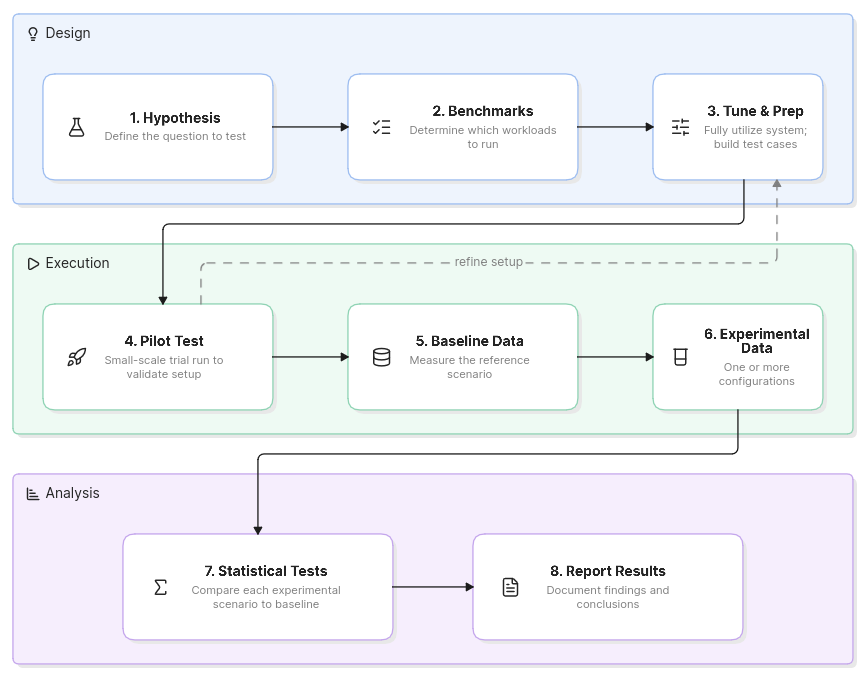
\includegraphics[width=\linewidth]{workflow.png}
    \caption{Workflow diagram listing the general steps and ordering between steps}
    \label{fig:workflow}
\end{figure}

\subsubsection{Define the Hypothesis and Equivalence Threshold}

This framework is best at testing hypotheses such as "Implementing an in-band 
monitoring system will have a measurable effect on system performance" or 
"Changing option X on the monitoring system will reduce system overhead" or 
"The new version of the monitoring system will reduce system overhead".

An equivalence threshold should also be defined before data collection.
This threshold specifies the maximum difference between the baseline and experimental 
conditions that is considered practically negligible. This value should be guided by
an examination of system requirements. For example, a system's operator could determine
that they are willing to tolerate at most \$5000 in additional cost per day and
that this is equivalent to 1\% additional overhead on the system.

Both the hypothesis and the equivalence threshold should be specified before 
conducting the experiment to avoid interpreting them retrospectively based on the 
observed results.

\subsubsection{Selecting Benchmarks}
We begin by selecting benchmarks to run. The benchmarks will vary by system. 
As guidance, we suggest that 
these benchmarks include at least those used in system acceptance. Additionally, 
we suggest using any benchmarks intended to be small scale simulations of 
workloads the system is expected to run.
Finally, we suggest HPL\cite{dongarraLINPACKBenchmarkPresent2003} and 
HPCG\cite{herouxNewMetricRanking2013} as good benchmarks. HPL is designed to 
measure the computational capacity of a system, while HPCG provides a 
more holistic measurement.

\subsubsection{Tuning Benchmarks and Preparing Test Cases}

The benchmarks are then tuned to the experimental system. 
We anticipate that in many cases, such tuning will already have 
been performed as part of system acceptance. 
Additionally, test cases are defined, written down, and prepared. These cases 
reflect the experimental 
condition(s) and must be identical except for the element under test.
For example, if testing the overhead of a potential system-wide monitoring system,
a user might prepare two images which are identical, except that one does not have the
monitoring software installed, while the other does.

\subsubsection{Pilot Test}

Next, we must determine the sample size required for statistically significant 
results. A small pilot study of the benchmarks is run. This includes running 
each of the tests under the baseline and experimental conditions a 
predetermined number of times. 

The gathered data is then used to perform power analysis.
By default, power analysis is performed using the method of Happ et al.\cite{happOptimalSampleSize2019}, as this is appropriate for the Mann--Whitney U test 
used later when analyzing data. If a user plans to use a different statistical test 
when analyzing data, the method for power analysis must be changed to 
match and the reason for the change documented. Note that the 
method of Happ et al.\cite{happOptimalSampleSize2019} uses the pilot distributions to estimate the quantities required for Wilcoxon--Mann--Whitney sample-size planning. If another test is used, the corresponding sample-size method and required effect specification must also be documented.

The following parameters are default values for the power analysis:

\begin{table}[h!]
\centering
\begin{tabular}{| c | c |} 
    \hline
    Parameter & Value \\ [0.5ex] 
    \hline
    Repeats, each benchmark & 20 \\ 
    \hline
    $\alpha$ (alpha) & 0.05 \\ 
    \hline
    Power & 0.8 \\
    \hline
    Equivalence Threshold & site-specific \\
    \hline
\end{tabular}
\caption{Default parameters used for power analysis}
\label{table:power_params}
\end{table}

These parameters regulate the chance of errors. Setting $\alpha$ to 0.05
indicates a maximum risk of a Type I (false positive) of 5\%. Setting Power
to 0.8 indicates a maximum risk of a Type II error (false negative) of 20\%.
Any change in these parameters must be documented. 

The result of power analysis serves as a minimum number of tests to run. The user may choose to 
run more, but must decide how many tests to run before gathering data.

\subsubsection{Gathering Data}

In order to gather statistically significant data, the benchmarks are run 
for at least as many repetitions as required by the power analysis and a
performance metric gathered from each run. The performance 
metric need not be the same between all benchmarks, but must be consistent 
for each benchmark. 
Overhead is calculated such that a positive number always indicates an
experimental condition performed worse than the base condition it is being
compared to.
Example performance metrics 
include runtime, FLOPs, and I/O operations per second, but will vary based on 
the benchmark.
If the runtime environment may change over time (for example, the coolant temperature
to the system varies with the outside temperature), runs should be interleaved, 
either in small groups or individually, with
the order randomized.
Benchmarks are then run a predetermined number of times under each 
experimental condition and the performance metric from each stored.

\subsubsection{Analysis}

Once sufficient data is collected, the percent overhead is calculated.
If the performance metric will be reduced when a benchmark performs worse, use:

\(overhead (\%) = \frac{mean(baseline)-mean(experimental)}{mean(baseline)}*100\)

Otherwise, if the metric increases when a benchmark is worse-performing, use:

\(overhead (\%) = -\frac{mean(baseline)-mean(experimental)}{mean(baseline)}*100\)

The significance of the result is then determined by testing two hypotheses.
By default, we use the Mann--Whitney U test, a nonparametric test for two independent
samples. Unlike the Student's t-test, it does not require normally distributed input data.
This is useful for performance measurements because, as Hoefler and Belli
\cite{hoeflerScientificBenchmarkingParallel2015} note, normal distributions are uncommon
in computer-performance data. Users of the framework may select another statistical test,
but must document the replacement and justify why it is appropriate for the experimental design.

We apply the test to two hypotheses. In the first, the hypothesis is that the 
distribution of values in the baseline and experimental conditions differs. Conversely,
the null hypothesis is that the values from the baseline and experimental conditions 
have the same distribution.
These are the hypotheses evaluated by the two-sided Mann--Whitney U test.

In the second analysis, we assess equivalence using the predefined margin $\theta$.
Following the general two one-sided tests (TOST) principle\cite{lakensEquivalenceTestingPsychological2018},
the implementation shifts the baseline performance distribution by the lower and upper
equivalence limits and applies two one-sided Mann--Whitney U tests. Equivalence is concluded
only when both one-sided null hypotheses are rejected; operationally, we report the larger
of the two p-values. This procedure tests whether the experimental performance lies within
the predefined equivalence region under the location-shift interpretation used by the
implementation. The value and units of $\theta$, and any departure from this default
procedure must be documented.

\subsection{Reporting Results}

To support comparison between sites, users of the methodology shall report the configuration used to run the benchmark. We propose four cumulative reporting tiers: \textbf{Bronze}, the minimum information required to report a result; \textbf{Silver}, results that are somewhat comparable between sites but may not be replicable; \textbf{Gold}, results that are replicable although setting up a reproduction environment may be difficult; and \textbf{Platinum}, full reproducibility of the test environment with reduced effort compared to Gold. Additional information may be reported where relevant, and information above Bronze may be placed in an appendix or associated artifact.

\textbf{Bronze} reporting includes: (1) a description of the base case and how each experimental case differs from it; (2) the benchmarks and their configurations; (3) a result summary including measured overhead, statistical methods (if different from those described here), and measures of statistical significance; (4) hardware details including manufacturer, CPU count and model, RAM speed and amount, storage, network, and other relevant system information; (5) job-manager name and version; (6) operating-system name and version; and (7) the name and version of any software changed between the base and test cases, together with any non-default configuration or configuration file. Measured overhead should be reported as percent overhead at the stated collection frequency. We use 1~Hz as the default because it should be achievable by most monitoring software and is frequent enough to expose overhead; any change in collection rate and its rationale must be documented. Ideally, collection and transmission to aggregation servers occur at the same rate.

\textbf{Silver} adds the performance measurement from every benchmark run, the software or code used for statistical analysis (including name/version or citation as appropriate), and benchmark configuration files.

\textbf{Gold} adds the information needed to reconstruct the runtime environment closely: a list of installed software versions (for example, from \texttt{dnf list installed}, \texttt{yum list installed}, or \texttt{apt list --installed}, together with \texttt{/etc/os-release} where available), plus network and storage system specifications and version numbers. These items are separated from Silver because some may require administrative access.

\textbf{Platinum} adds the information needed for the most complete reproduction: full scripts and code used to run tests and statistics (excluding publicly available benchmark code or code that cannot be shared under its license), workload-manager configuration files, a list and contents/diffs of changed system files unless disclosure would create a security issue or the change was made automatically by software, and configuration files or details of all changed network and storage options. The changed-file list may, for example, be collected using \texttt{rpm -Va}; alternatively, an image or other reproducible method of creating the compute-node image may be provided. Platinum reporting should allow complete reproduction and validation of the experiment.

\section{Implementation} \label{implementation}

To facilitate practical use and reproducibility of the proposed framework, we 
provide a reference implementation\cite{HPCNexusLabImpactofMonitoringonHPCWorkloads}. This reference uses 
reFrame\cite{karakasisRegressionFrameworkChecking} to manage running benchmarks,
then performs analysis in a Jupyter notebook.
reFrame was selected as a base software because it can easily be installed and 
run on most systems. It is 
distributed as a Python package, which may be installed in a per-user virtual environment 
and therefore does not require administrative access to install. Further, it 
does not require alteration of existing job managers to use. Instead, it is 
configured to use the user's existing access and therefore may be run without 
the assistance of the systems administrators. Finally, reFrame brings several 
convenient functions, including automatic compilation of test code and storage 
of results.

In order to demonstrate this framework, we run it with four experimental 
conditions:
\begin{itemize}
    \item Using LDMS with the configuration file in the associated artifacts\cite{HPCNexusLabImpactofMonitoringonHPCWorkloads}
    \item Using HPCPerfStats with the configuration file in the associated artifacts\cite{HPCNexusLabImpactofMonitoringonHPCWorkloads}
    \item Collecting metrics from the BMC with a custom script 
    (contained in the associated artifacts\cite{HPCNexusLabImpactofMonitoringonHPCWorkloads})
    \begin{itemize}
        \item with a helper daemon running in the OS to collect additional metrics
        \item without the helper daemon running in the OS
    \end{itemize}
\end{itemize}
The benchmarks run under Slurm on a HPE DL360 Gen 10 with two Intel Xeon Gold 
5120 processors and 16 GiB DDR4 2133 MHz RAM. The system BMC is an iLO5 running firmware 3.19.
The network was 1 GbE, provided by the built-in network interface using 
a Broadcom NetXtreme BCM5719. Storage was provided by the built-in RAID 
controller (based on an Intel C620) and an Intel SSDSA2BW16 SSD. This node was 
the only worker in a Slurm 26.05.2 cluster and ran Rocky Linux 9.8. The Slurm 
controller was a KVM virtual machine which provided an NFS home 
filesystem, connected to the worker via an unmanaged network hub.

\subsection{Experimental Hypothesis}

We begin by stating our hypotheses:
\begin{enumerate}
    \item The use of in-band monitoring systems (LDMS and HPCPerfStats) will increase overhead in an HPC 
    system
    \item The use of out-of-band monitoring via the BMC (with and without an OS-level helper daemon) will remain within the predefined equivalence bound
\end{enumerate}
Before conducting the analysis, we set a threshold for equivalence. This threshold is the maximum 
change between the baseline and an experiment that is considered equivalent. It
will vary from system to system and depends on the tolerance of overhead on the system.
For the purposes of demonstration, we set this at 0.5\% for our tests.
Users of the framework will likely wish to adjust this value based on their
needs. For example, academic systems may wish to increase it, as users will likely want 
significant monitoring data, rather than being performance focused. In contrast, 
systems with real-world job deadlines (such as those used for weather forecasting) may wish a lower value, as they have 
strict limits on job runtime.

\subsection{Selecting Benchmarks}

In order to keep this evaluation simple, we focus on single-node CPU 
benchmarks. Because the software monitoring systems must use the CPU, we 
believe this is the element of the system most likely to show an effect from 
monitoring software. Further, Faasse et al.\cite{faasseOutBandPerformance2020}
questioned whether BMC-based monitoring would impact the performance of a CPU-based
benchmark. This is an important question for users of BMC-based monitoring, and
we test this case in order to generate additional data.
We selected HPL\cite{dongarraLINPACKBenchmarkPresent2003} and the EP (Embarrassingly Parallel) and SP (Scalar Penta-diagonal solver) benchmarks from the NPB suite\cite{NASParallelBenchmarksa} as our test benchmarks. 

HPL is a well-known and often run measurement of the capacity of a system to 
perform floating point operations (FLOPS). The EP benchmark is 
CPU-focused and provides an "estimate of the
upper achievable limits for floating point performance"\cite{NASParallelBenchmarks}
and includes minimal interprocess communication. We believe that if the CPU 
must perform additional work for the monitoring system, that will appear as a 
slowdown or reduction in performance of the HPL and EP benchmarks.
We run HPL with a custom configuration, included in the associated artifacts\cite{HPCNexusLabImpactofMonitoringonHPCWorkloads}. On 
the specified hardware, this takes approximately 10 minutes to run.
For EP, we selected the D and E problem sizes of the EP benchmark. The D size runs 
quickly (about 50 to 60 seconds on our test hardware), while the E takes 
approximately 15 minutes.

In contrast, SP was selected because it makes use of various resources. We do not 
expect it to fully utilize the CPU and therefore expect to see no impact on it 
as the monitoring configuration changes. It is thus a contrasting workload.
We 
select the C size, which runs in approximately 280 seconds (4 minutes 40 seconds).
Together, these benchmarks provide complementary workload characteristics, allowing us to evaluate monitoring overhead under both compute-focused and less CPU-constrained conditions.

\subsection{Tuning Benchmarks and Preparing Test Cases}

The EP benchmark was configured to run 56 tasks, equal to the number of hardware
threads available to the operating system. HPL also used 56 tasks with the configuration
provided in the associated artifact, but was not tuned for peak HPL performance. SP was not tuned. 
Finally, we select FLOPS (floating point operations per second) as our performance benchmark for HPL and 
millions of operations per second (Mops/s) as our performance benchmark for EP and SP. This 
value is automatically calculated by the benchmarks.
The SP benchmark requires a square number of tasks. In our case, 
it was run with 49 tasks, using 49 hardware threads. This left 7 hardware
threads for other work on the system. 
This simulates a condition in which the running workload is bound by a resource 
other than CPU time.

In order to test the effect of in-band monitoring, we evaluate two different 
monitoring systems: HPCPerfStats and LDMS. The configuration used for each is
available in the associated artifacts\cite{HPCNexusLabImpactofMonitoringonHPCWorkloads}.
HPCPerfStats was configured 
with the default collection (which includes CPU statistics, block device IO, and \texttt{/proc}
information), while LDMS was configured to collect using the 
\texttt{meminfo}, \texttt{coretemp}, \texttt{loadavg}, \texttt{procnet}, 
\texttt{procstat2}, and \texttt{vmstat} modules. Both were configured to collect 
and send data to a central server once per second (1 Hz).

In order to test the effect of BMC-based out-of-band monitoring, we use the BMC 
built into the compute node, an HPE iLO5. Because this is part of the hardware, 
we cannot test any alternatives without fundamentally changing the hardware.
The HPE iLO5 provides the ability to measure CPU, I/O and memory bus utilization 
via \texttt{amsd} (Agentless Management Service daemon)\cite{HPEAgentlessManagement},
a daemon which is installed on the operating system of the node.
Unfortunately, it appears that on the system used, \texttt{amsd} only provides 
this information once every 20 seconds. We nonetheless install it in order to 
maximize the potential impact of monitoring via the BMC. We test two BMC cases 
- one with \texttt{amsd} running and one without \texttt{amsd} running. Thus, we 
can separate any effect of \texttt{amsd} from monitoring with just the BMC.

BMC sensor data was collected from the BMC once per second using Redfish.
In the \texttt{amsd} case, this collection includes the \texttt{amsd} data, although it changes only once 
every 20 seconds. The 
script and URLs used for collection are available in the 
associated artifacts\cite{HPCNexusLabImpactofMonitoringonHPCWorkloads}. The collector ran on the Slurm admin node.
Finally, we script shifting between the five test cases (no monitoring, 
HPCPerfStats, LDMS, BMC with \texttt{amsd}, and BMC without \texttt{amsd}) in 
order to ensure consistent system state.
This script is available in the associated artifacts\cite{HPCNexusLabImpactofMonitoringonHPCWorkloads}.

\subsection{Pilot Test}

After tuning the benchmarks and defining the experimental conditions, we conduct 
a pilot study to estimate the variability of benchmark performance and determine 
the amount of data required for the full experiment. For the code used 
to run these tests, please see the artifacts accompanying this paper\cite{HPCNexusLabImpactofMonitoringonHPCWorkloads} .

For the pilot study, we run 20 iterations of each benchmark under the baseline 
(no monitoring) and each of the experimental conditions. We assume each 
run of the benchmark is independent. Each benchmark controls the entire machine 
while running and no two benchmarks ever run at the same time. They thus should
not influence each other. Additionally, the physical environment is climate controlled to reduce environmental variation.
We then perform a 
power analysis using the following values to determine the minimum number of 
runs of each benchmark are required. The Jupyter notebook used to perform power 
analysis is included in the associated artifacts\cite{HPCNexusLabImpactofMonitoringonHPCWorkloads}.

We use the default parameters for the power analysis. For the purposes of
demonstration, we pick 0.005 (0.5\%) as our equivalence threshold.

\subsection{Gathering Data}


Following the pilot study, we perform power analysis to determine the required 
sample size for each benchmark and monitoring condition. Additional experimental 
cycles (if needed) are then collected until the required sample size is reached. 
Power analysis results can be found in section 
\ref{results}. 

\subsection{Analysis}

Finally, analysis was performed using the Jupyter notebook, available in the
associated artifacts\cite{HPCNexusLabImpactofMonitoringonHPCWorkloads}. The analysis is presented in section 
\ref{results}. This includes two statistical tests: a Mann--Whitney U test to 
determine if there is a statistically significant difference between the base 
and test cases and two one-sided Mann--Whitney U tests to determine if the effect is within the 
equivalence bound chosen earlier. Notably, the use of two statistical tests can result 
in both tests being statistically significant. In this case, there is a statistically
detectible difference between the base and experimental cases. However, that difference 
is small enough to satisfy the equivalence criterion. Therefore, based on the 
predetermined equivalence bound, the difference in performance is not practically 
meaningful.

\section{Results} \label{results}
This section reports the results obtained using the proposed methodology. We first 
present the pilot-study and power-analysis results used to determine the required 
sample sizes, followed by the results of the full monitoring-overhead evaluation.

\subsection{Pilot Study}

We performed a pilot study to determine how many repetitions of each experiment 
were required for statistically significant results. Table \ref{table:power_analysis}
contains the raw results of the power analysis.

\begin{table}[h!]
\centering
\begin{tabular}{| c | c | c |} 
    \hline
    Test & Indicated samples required & Erroneous samples required \\ [0.5ex] 
    \hline
    EP, size D & 20 & 197\\ 
    \hline
    EP, size E & 80 & 103\\ 
    \hline
    HPL & 52 & 118 \\
    \hline
    SP & 20 & 192 \\
    \hline
\end{tabular}
\caption{Number of runs indicated by power analysis, including sample counts indicated by an earlier erroneous calculation. All values are per test case.}
\label{table:power_analysis}
\end{table}

Our initial power-analysis code contained a bug and overestimated the number of
repetitions required. Because most of the additional data had already been collected when
the error was discovered, those runs are retained in the analysis. Two conditions remain
at the 20-run pilot size---EP size E with HPCPerfStats and HPL with BMC monitoring without
\texttt{amsd}---which is below the corrected benchmark-level counts shown in
Table \ref{table:power_analysis}; these two cells should therefore be interpreted cautiously.


\subsection{Full Study}\label{full_results}

Our full study showed the following results, organized by test case. 
All of our performance measurements are reduced as performance decreases, so
overhead is calculated as:

\(overhead (\%) = \frac{mean(baseline)-mean(experimental)}{mean(baseline)}*100\)

A positive 
number indicates the job slowed by that much, while a negative number indicates 
the job ran faster under the test condition.

\begin{table*}[!t]
\centering
\footnotesize
\setlength{\tabcolsep}{4pt}
\begin{tabular}{llrrrr}
\hline
Monitoring condition & Test case & Overhead & $n$ & $p_{\mathrm{diff}}$ & $p_{\mathrm{eq}}$ \\
\hline
HPCPerfStats & EP, size D & 0.38\% & 200 & 0.029 & 0.015 \\
             & EP, size E & 2.03\% & 20  & 0.007 & 0.988 \\
             & HPL        & 0.07\% & 125 & 0.553 & $8.85\times10^{-22}$ \\
             & SP, size C & -0.185\% & 200 & 0.477 & $3.99\times10^{-20}$ \\
\hline
LDMS         & EP, size D & 0.11\% & 200 & 0.519 & 0.0004 \\
             & EP, size E & 0.05\% & 110 & 0.803 & 0.026 \\
             & HPL        & 0.09\% & 125 & 0.019 & $2.03\times10^{-22}$ \\
             & SP, size C & -0.073\% & 200 & 0.373 & $2.47\times10^{-20}$ \\
\hline
BMC without \texttt{amsd} & EP, size D & 0.198\% & 200 & 0.446 & 0.001 \\
             & EP, size E & -0.077\% & 110 & 0.958 & 0.002 \\
             & HPL        & 0.015\% & 20 & 0.744 & $3.24\times10^{-8}$ \\
             & SP, size C & 0.110\% & 200 & 0.893 & $9.77\times10^{-21}$ \\
\hline
BMC with \texttt{amsd} & EP, size D & 0.07\% & 200 & 0.212 & 0.001 \\
             & EP, size E & 0.04\% & 110 & 0.473 & 0.026 \\
             & HPL        & 0.27\% & 125 & $4.06\times10^{-5}$ & $7.75\times10^{-21}$ \\
             & SP, size C & -0.09\% & 200 & 0.507 & $6.61\times10^{-21}$ \\
\hline
\end{tabular}
\caption{Monitoring-overhead results. $p_{\mathrm{diff}}$ is the two-sided Mann--Whitney U-test p-value for a difference; $p_{\mathrm{eq}}$ is the larger p-value from the two one-sided Mann--Whitney equivalence tests using the 0.5\% bound.}
\label{table:results_all}
\end{table*}

Overall these results show HPCPerfStats has a measurable impact greater than 0.5\% on EP size E, but not EP size D, HPL or SP.
LDMS has a measurable impact on HPL, but overhead is in all cases less 
than the equivalence threshold. Overhead for the BMC without \texttt{amsd} is
in all cases under the equivalence threshold. The same is true for the BMC with \texttt{amsd},
except that there is a statistically detectable impact on HPL.
Histograms for all baseline and monitoring-condition measurements are provided 
in the associated artifacts\cite{HPCNexusLabImpactofMonitoringonHPCWorkloads}.
Finally, the BMC without \texttt{amsd} cases for EP size D and E and HPL 
were run at a different time than the other EP size D and E and HPL tests. A 
separate baseline data set was collected for each of these tests to ensure that
any measured effect was due to the monitoring system and not a long-term 
environmental drift -- although we know of no cause for such drift.

% SP 
% filter:  benchmark==\"sp\"

% HPCPerfStats: sp_test: mops_total: 200/200 experimental/base samples
%     t=19177.0 
%     p-value, different=0.4768251579721854
%     p-value, equivalent=3.9883727696668686e-20 (lower: 2.574758539611659e-27, upper: 3.9883727696668686e-20)
%     baseline:     mean: 5217.51625, stddev: 125.1144830722547
%     experimental: mean: 5227.2168, stddev: 120.1168364375286
%     difference: -0.18592275587067844%
% LDMS: sp_test: mops_total: 200/200 experimental/base samples
%     t=21031.0 
%     p-value, different=0.3727540078311695
%     p-value, equivalent=2.4683206102324298e-20 (lower: 2.0458966840847171e-22, upper: 2.4683206102324298e-20)
%     baseline:     mean: 5217.51625, stddev: 125.1144830722547
%     experimental: mean: 5221.2891500000005, stddev: 119.00654668873267
%     difference: -0.07231218494050393%
% BMC_with_helper: sp_test: mops_total: 200/200 experimental/base samples
%     t=20768.5 
%     p-value, different=0.5065121446458085
%     p-value, equivalent=6.6132078675193026e-21 (lower: 1.3870376588918563e-25, upper: 6.6132078675193026e-21)
%     baseline:     mean: 5217.51625, stddev: 125.1144830722547
%     experimental: mean: 5222.3911499999995, stddev: 122.47626481558581
%     difference: -0.09343334579935036%
% BMC_no_helper: sp_test: mops_total: 200/200 experimental/base samples
%     t=19844.0 
%     p-value, different=0.893007936254366
%     p-value, equivalent=9.766562707602024e-21 (lower: 9.766562707602024e-21, upper: 7.971348877238725e-23)
%     baseline:     mean: 5217.51625, stddev: 125.1144830722547
%     experimental: mean: 5211.846949999999, stddev: 127.96516329531839
%     difference: 0.10865898117711614%


% HPL
% filter: and benchmark==\"hpl\""
% separate baseline for BMC_no_helper, run separately and use baseline test=="no_monitoring_bmc_only"

% LDMS: hpl_test: gflops: 125/125 experimental/base samples
%     t=9150.5 
%     p-value, different=0.019086376912192036
%     p-value, equivalent=2.0261798325084883e-22 (lower: 2.0261798325084883e-22, upper: 9.47230058266034e-30)
%     baseline:     mean: 11.678655999999998, stddev: 0.0858836519018609
%     experimental: mean: 11.667816, stddev: 0.09603610854256858
%     difference: 0.09281889970899207%
% HPCPerfStats: hpl_test: gflops: 125/125 experimental/base samples
%     t=8151.5 
%     p-value, different=0.5530024801114728
%     p-value, equivalent=8.847588202346536e-22 (lower: 8.847588202346536e-22, upper: 1.2716206119267685e-29)
%     baseline:     mean: 11.678655999999998, stddev: 0.0858836519018609
%     experimental: mean: 11.669936000000003, stddev: 0.09750952724734135
%     difference: 0.07466612596513636%
% BMC_with_helper: hpl_test: gflops: 125/125 experimental/base samples
%     t=10156.0 
%     p-value, different=4.059337869664996e-05
%     p-value, equivalent=7.752060280606334e-21 (lower: 7.752060280606334e-21, upper: 3.380360605772211e-30)
%     baseline:     mean: 11.678655999999998, stddev: 0.0858836519018609
%     experimental: mean: 11.647087999999998, stddev: 0.1360691010332618
%     difference: 0.2703050762005495%
% BMC_no_helper: hpl_test: gflops: 20/20 experimental/base samples
%     t=212.5 
%     p-value, different=0.7442759394630934
%     p-value, equivalent=3.242858844342788e-08 (lower: 3.242858844342788e-08, upper: 3.242858844342788e-08)
%     baseline:     mean: 11.704749999999999, stddev: 0.004592112803493169
%     experimental: mean: 11.702950000000001, stddev: 0.006344091739563577
%     difference: 0.015378372028429326%
    
% EP-E
% filter: (\"jobsize\" not in locals() or jobsize==\"E\") and (\"benchmark\" not in locals() or benchmark==\"ep\")
% separate baseline for BMC_no_helper, run separately and use baseline test=="no_monitoring_bmc_only"

% LDMS: ep_test: mops_total: 110/110 experimental/base samples
%     t=6168.0 
%     p-value, different=0.8034314239946994
%     p-value, equivalent=0.003402698676263021 (lower: 0.003402698676263021, upper: 0.0013657743328025459)
%     baseline:     mean: 2751.204454545455, stddev: 53.001269497426605
%     experimental: mean: 2749.8882727272726, stddev: 55.85835576558541
%     difference: 0.04784020380629766%
% BMC_with_helper: ep_test: mops_total: 110/110 experimental/base samples
%     t=6389.0 
%     p-value, different=0.47333163111944443
%     p-value, equivalent=0.02584392604732822 (lower: 0.02584392604732822, upper: 0.0003768375280283294)
%     baseline:     mean: 2751.204454545455, stddev: 53.001269497426605
%     experimental: mean: 2750.051636363637, stddev: 50.09867173937437
%     difference: 0.041902308638435415%
% HPCPerfStats: ep_test: mops_total: 20/20 experimental/base samples
%     t=300.0 
%     p-value, different=0.007113494035772574
%     p-value, equivalent=0.9880484270662208 (lower: 0.9880484270662208, upper: 0.0010696306978677111)
%     baseline:     mean: 2755.29, stddev: 51.02268436685783
%     experimental: mean: 2699.3334999999997, stddev: 68.73056730996767
%     difference: 2.030875152887726%
% BMC_no_helper: ep_test: mops_total: 110/110 experimental/base samples
%     t=6024.5 
%     p-value, different=0.9577643418371677
%     p-value, equivalent=0.001633881602287935 (lower: 0.001633881602287935, upper: 0.001328299734739213)
%     baseline:     mean: 2755.0333636363634, stddev: 51.02061690723703
%     experimental: mean: 2757.144818181818, stddev: 47.114301375037385
%     difference: -0.07663989022143303%
    
% EP-D
% filter: jobsize==\"D\" and (\"benchmark\" not in locals() or benchmark==\"ep\")
% separate baseline for BMC_no_helper, run separately and use baseline test=="no_monitoring_bmc_only"

% LDMS: ep_test: mops_total: 200/200 experimental/base samples
%     t=20746.5 
%     p-value, different=0.5187658078357676
%     p-value, equivalent=0.00043891476101 (lower: 0.00043891476101, upper: 1.9827343861704227e-06)
%     baseline:     mean: 2755.66725, stddev: 43.852086483284914
%     experimental: mean: 2752.5066500000003, stddev: 45.722306462792325
%     difference: 0.11469454448826157%
% HPCPerfStats: ep_test: mops_total: 200/200 experimental/base samples
%     t=22528.5 
%     p-value, different=0.028773080067512828
%     p-value, equivalent=0.014818634697815958 (lower: 0.014818634697815958, upper: 6.069307439909863e-10)
%     baseline:     mean: 2755.66725, stddev: 43.852086483284914
%     experimental: mean: 2745.0620999999996, stddev: 50.23690684735676
%     difference: 0.38484871495280576%
% BMC_with_helper: ep_test: mops_total: 200/200 experimental/base samples
%     t=18557.0 
%     p-value, different=0.21214701392653124
%     p-value, equivalent=0.0014733275449542271 (lower: 2.5298687608559007e-07, upper: 0.0014733275449542271)
%     baseline:     mean: 2755.66725, stddev: 43.852086483284914
%     experimental: mean: 2753.87505, stddev: 64.90682870852264
%     difference: 0.06503687990630459%
% BMC_no_helper: ep_test: mops_total: 200/200 experimental/base samples
%     t=20882.0 
%     p-value, different=0.4457919222854053
%     p-value, equivalent=0.001671361735777248 (lower: 0.001671361735777248, upper: 2.340633720844604e-06)
%     baseline:     mean: 2755.66725, stddev: 43.852086483284914
%     experimental: mean: 2750.19565, stddev: 65.82953358924473
%     difference: 0.19855808062456937%


\section{Discussion} \label{discussion}

These results lead to some interesting conclusions. In some cases, we did 
observe meaningful overhead from running monitoring. Specifically, we 
found that running 
HPCPerfStats showed a 2.0\% overhead when running 
EP in size E.
In contrast, the overhead for both LDMS and BMC-based monitoring was within our 
predefined bound for equivalence for EP size E.

It is unclear why HPCPerfStats had a significant impact on EP size E 
while LDMS did not. 
One theory is the number of modules performing collection causes the impact. 
Validating this theory is beyond the scope of the current work.
In the tested installation, HPCPerfStats exposed 31 modules (although some hardware- and software-specific modules had no source from which to collect data), whereas the LDMS configuration enabled 6. Perhaps one (or more) of these modules have significant 
system impact. Benchmarking individual modules of monitoring systems is beyond 
the scope of this paper. However, the framework proposed within this paper 
could be used for such benchmarking.

No monitoring system creates overhead on HPL greater than 0.5\%.
BMC-based monitoring with the \texttt{amsd} daemon and LDMS show statistically detectable
differences of 0.27\% and 0.09\%, respectively, while the 0.07\% HPCPerfStats difference
is not statistically detectable ($p=0.553$). All four HPL conditions remain within the
predefined 0.5\% equivalence bound.

As expected, SP (which in our tests left 7 hardware threads on the system idle) shows an effect
within the predefined 0.5\% bound in all cases. This is consistent with, 
but does not confirm our hypothesis
that the monitoring daemon impact is due to CPU contention.

The results on a per-benchmark basis do indicate that monitoring systems can 
have significant overhead. They also show that the overhead varies
based on the combination of monitoring system, workload, and workload 
configuration. In turn, this emphasizes the need for administrators considering 
a monitoring system to test it with workloads/benchmarks that reflect their 
system and uses. What is right for one system may not be right for another. 
In turn, a framework like the one laid out in this work is therefore critical 
to allow systems administrators to systematically evaluate monitoring for each 
system.

Shifting from individual benchmarks, we are able to draw some conclusions about 
the monitoring systems themselves. Our results are consistent with low practical overhead from LDMS on the tested platform and workloads. In all cases, LDMS remained within our 0.5\% equivalence bound.
Further statistical 
tests (using a smaller equivalence bound) could more precisely define the overhead.

Finally, in the tested configuration, monitoring via the BMC 
does not have any meaningful overhead. The largest observed 
overhead for BMC-based monitoring (and the only one measured as 
statistically significant) was a 0.27\% impact on HPL when 
running monitoring via the BMC with the OS-based helper daemon. This is
consistent with additional overhead when using an OS-based helper daemon.
However, without the OS-level daemon running, BMC-based 
monitoring contributed negligible overhead. Further experiments are 
necessary to determine whether this remains true under other test conditions.
Tests runs in more hardware configurations could determine whether 
BMC-based monitoring is a good monitoring choice for 
overhead-sensitive environments.

\section{Limitations and Future Work} \label{futurework}

The use of a single node in these tests limits the generalizability of the results.
These results may not directly generalize to jobs running across multiple nodes, where the 
network may have an impact. Nor are they applicable when a shared storage system
is be used. Hypothetically, the effects observed here might
be lost in the network jitter when running multi-node versions of the 
same benchmarks. Conversely, additional jitter caused by monitoring collecting data 
at different times on different nodes could cause these effects to be larger in
multi-node jobs. Real-world testing is necessary to test these effects in 
multi-node systems.

The study also evaluates a single BMC implementation and a single-node platform.
The HPL configuration was not tuned for peak HPL performance, so its results should be
interpreted as applying to the tested configuration rather than to an optimized HPL run.
In the supplied implementation, conditions were executed in a fixed order within each cycle; systematic time-dependent drift could therefore be confounded with condition, and future experiments should randomize or counterbalance the order.
Finally, the use of a fixed 1 Hz collection rate, while helpful
for comparability, means that the impact may change with other collection rates.
Future work could examine all of these limitations by evaluating 
these same benchmarks across different hardware and software configurations, including multi-node configurations.
It will also consider other workload types, including GPU- and accelerator-focused benchmarks.

The accompanying code present in HPC Nexus Lab GitHub \cite{HPCNexusLabImpactofMonitoringonHPCWorkloads} 
contains an example of running the benchmarks in cycles. The framework is
not currently capable of performing statistical analysis when the test 
conditions vary over time.
% Future work could
% extend this framework to remove that limitation.
% For example,
% a software upgrade during data gathering could affect the results, as could a 
% change in the temperature of cooling water.
Future work will
extend the statistical analysis elements of the sample implementation to
compensate for changes in the computing environment that occur over time.

Additionally, future work will examine the applications of
out-of-band monitoring data. Given the low overhead observed for out-of-band monitoring in our experiments, we wish to explore how
this data can be used to better monitor running systems and jobs. For instance, can it 
be used to detect stalled jobs? Can it be used to determine what kinds of jobs
are running on a system? Can it be used for early detection of hardware 
failures?

\section{Conclusion} \label{conclusion}

This work contributes a methodology for measuring the impact of various 
monitoring systems and configurations on the performance of HPC systems as well as providing 
various levels of reporting in order to encourage reproducibility. Further, it 
contributes a reference implementation of this methodology in order to assist 
future usage by others. It then 
applies this methodology to determine whether HPCPerfStats, LDMS and 
BMC-based monitoring have a meaningful overhead. Findings include an observed overhead of up to 2.0\% for HPCPerfStats, whereas
LDMS and BMC-based monitoring remained within the predefined 0.5\% equivalence margin
across the evaluated workloads. The two conditions retained at the 20-run pilot size should
be interpreted cautiously. To our knowledge, this provides one of the first statistically
structured evaluations of BMC-based monitoring overhead on HPC workloads.
More broadly, these results demonstrate the value of a consistent and statistically rigorous methodology for evaluating monitoring overhead across different HPC workloads and monitoring configurations.

\section*{AI Use Disclosure}
The Generative AI tool (ChatGPT 5.5) is used to assist with language editing,
consistency checking, and bibliographic metadata verification. All experiments, code, statistical calculations, references, and final manuscript content were performed, reviewed and verified by the authors, who take responsibility for the submitted work.

\bibliography{HPC-ODA_paper}

\end{document}
